\chapter{State Space Models}
\label{chap:two}


Applying the Kalman Filter to a system requires an understanding of state space models. A state space model represents a system's inputs, outputs, and states by describing a series of first order differential equations. A linear continuous state space system has a general form of 
\begin{align*}
&\dot x(t)= A x(t) + B u(t) +w(t) \quad &\text{(system)}, \\
&y(t) = H x(t) +v(t) \quad &\text{(observation)} ,
\end{align*}
where $x$ is the state vector, $A$ is a square transformation matrix, $B$ is the input matrix, $u$ is a system input, $w$ is the process noise vector, $y$ is the transformed prediction, $H$ is the observation matrix, $v$ is the measurement noise vector, and $t$ is time \cite{bolviken}. \\

\noindent For implementing Kalman Filters, the continuous state space system must be discretized into time steps, call it $k$. The general equation is given below as
\begin{align*}
& x_k= e^{At}x_{k-1} + \int_0^t e^{A(t-r))} B u_k dr + w_k \quad &\text{(system)}, \\
&y_k = H x_k + v_k  &\text{   (observation)} ,
\end{align*}
where $e^{At}$ is the matrix exponential of $A$  \cite{bolviken}.  Generally, the matrix exponential is very time-consuming to compute, especially if the matrix is not diagnolizable. In these cases, an alternative solution is to use Euler's method, which approximates the discretized system using small time steps, $t$,  as shown by 
\begin{align*}
& x_k= x_{k-1} + t f(x) + w_k  &\text{(system)}, \\
&y_k = H x_k + v_k  &\text{(observation)},
\end{align*}
where $f(x)$ is the state after it undergoes a transformation \cite{griffiths_higham_2011}. The accuracy of this discretization method is dependent on values of $t$, with smaller values performing better than larger values. A visualization of Euler's method with a $t$ value of 1 is given in Figure ~\ref{fig:EM}, with the red line being the discretized version of the continuous system represented by the blue line. The values $A_0, \hdots, A_4$ represents the discretized values at each time steps $0,\hdots, 4$ respectively. As the time steps increase, the discretized version becomes progressively further from the continuous system. A better discretization can be obtained by using smaller values of $t$. 

\begin{figure}[ht]
    \centering
    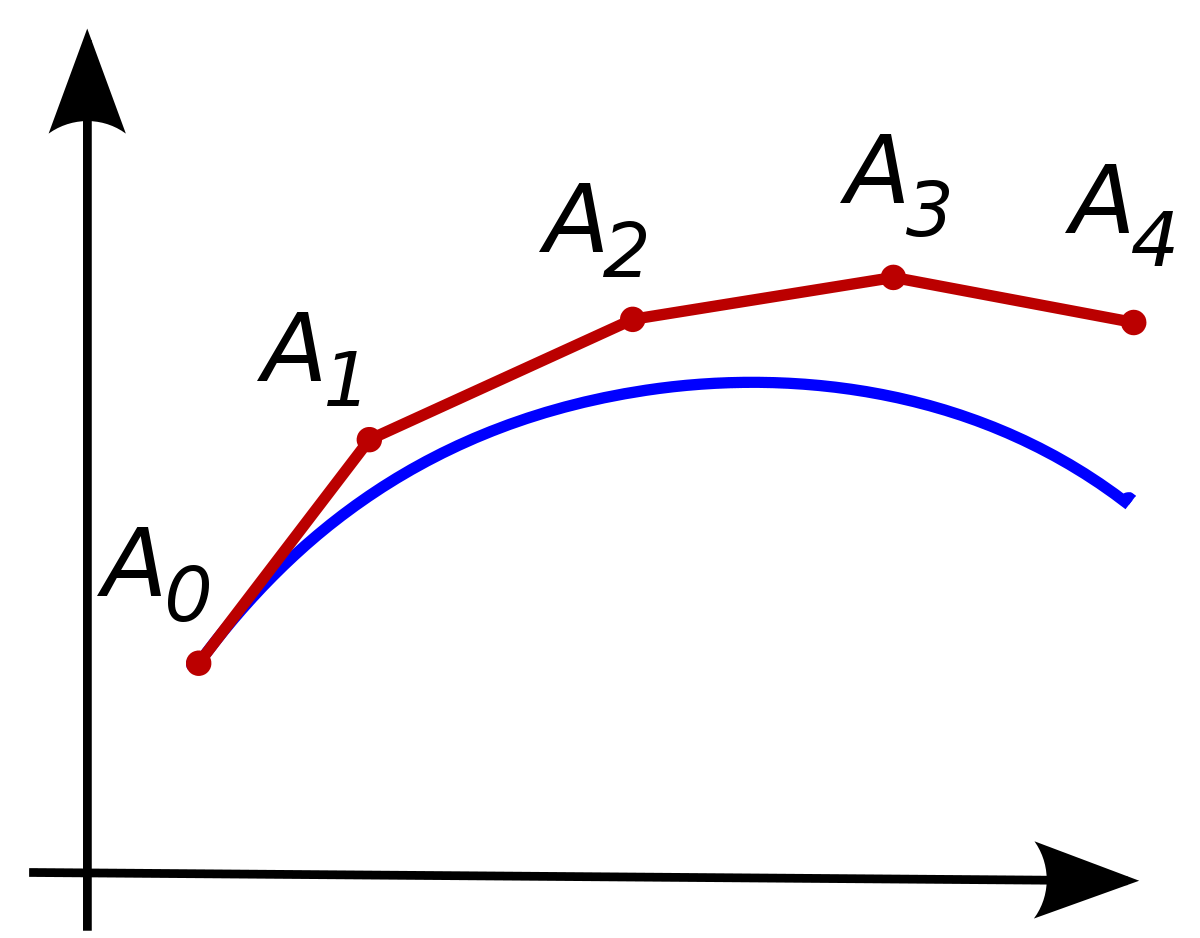
\includegraphics[scale = 0.15]{EM.png}
    \caption{This image taken from \cite{EM_image} visualizes how Euler's method of discretization works. Here, the blue line represents some nonlinear function and the red line visualizes discretization with a time step of 1. Since a time step of 1 is relatively large, one can see that the discretization becomes progressively further from true system as time goes on. To prevent this, consider using smaller time steps.}
    \label{fig:EM}
\end{figure}

\noindent In most of the examples that are explored in this thesis, computing the matrix exponential is inefficient and results in excessive computing time. Therefore, Euler's method will be mostly used for discretization. \\

\noindent To better understand converting systems in their state space forms using the matrix exponential, consider an example from \cite{bolviken} of a moving mass, call it $m$, under a force, call it $u(t)$. The goal of this system is to predict the mass's position and velocity given its previous position and velocity. Therefore, position and velocity are the two states in this system. From differential equations, recall that the position of the mass is denoted by $x(t)$, the velocity of the mass is denoted by $\dot{x}(t)$, and the acceleration is denoted by $\ddot{x}(t)$. According to Newton's second law of motion, the force exerted on an object is given by the equation $F=ma$, or
\begin{align*}
u(t)=m\ddot{x}(t).
\end{align*}

\noindent This is a second order differential equation. To convert it into its state space format, begin by transforming it into a first order differential equation by substituting $x_1(t)$ for $x(t)$ and $x_2(t)$ for $\dot{x}(t)$, resulting in
\begin{align*}
\dot{x}_1(t) = x_2(t), \\
\dot{x}_2(t) = \frac{u(t)}{m}.
\end{align*}

\noindent For the sake of simplicity, assume this system has no process or measurement noise. The state vector, $x$, containing both position and velocity, can now be rewritten as
$$
x=
\begin{bmatrix}
x_1(t)\\
x_2(t)
\end{bmatrix}.
$$

\noindent In order to predict the state of the system at the next time step, take the derivative of the state vector and rewrite it in vector-matrix form (which is possible because this system is linear), resulting in
$$
\dot x=
\begin{bmatrix}
\dot{x}_1(t)\\
\dot{x}_2(t)
\end{bmatrix}=
\begin{bmatrix}
x_2(t)\\
\frac{u(t)}{m}
\end{bmatrix}=
\begin{bmatrix}
0 & 1\\
0 & 0
\end{bmatrix} x +
\begin{bmatrix}
0\\
\frac{1}{m}
\end{bmatrix} u(t).
$$
Here, one can see how this form can be applied to the general linear state space model where $A = 
\begin{bsmallmatrix}
0 & 1\\
0 & 0
\end{bsmallmatrix} $ and $ B=[0, \frac{1}{m}]^T$. \\

\noindent For the sake of this example, assume that only the position of the mass is measurable. Therefore, the transformed prediction, $y$, is given by
$$
 y=
\begin{bmatrix}
x_1(t)\\
0
\end{bmatrix}=
\begin{bmatrix}
1 \\
0
\end{bmatrix} x=
x_1(t). $$

\noindent Now that the continuous state system is defined, it can be discretized. Since this example considers a simple linear system, the matrix exponential can be calculated  \footnote{Since this matrix is diagonalizable, the matrix exponential can be calculated by raising each element above the diagonal to the power of e.} as follows 

$$e^{At} =
\begin{bmatrix}
e^0& e^t \\
0 & e^0
\end{bmatrix}=
\begin{bmatrix}
1& T\\
0 & 1
\end{bmatrix},
$$

$$\int_0^t e^{A(t-r))}  e^{At} B u_k dr=
\int_0^t e^{A(t-r))}  \begin{bmatrix}
1& T\\
0 & 1
\end{bmatrix} 
\begin{bmatrix}
0\\
\frac{1}{m}
\end{bmatrix} u_k dt =
\int_0^t e^{A(t-r))}   \begin{bmatrix}
\frac{T}{m}\\
\frac{1}{m} 
\end{bmatrix} u_k dt =
\begin{bmatrix}
\frac{T^2}{2m}\\
\frac{T}{m}
\end{bmatrix} u_k.
$$
Now the discretized state space model can be written as 


\begin{align*}
x_k &=
\begin{bmatrix}
1& T\\
0 & 1
\end{bmatrix}x_{k-1}+
\begin{bmatrix}
\frac{T^2}{2m}\\
\frac{T}{m}
\end{bmatrix} u_k &\text{(system)}, \\
y_k &=
\begin{bmatrix}
1 \\
0
\end{bmatrix} x_k &\text{(observation)}.
\end{align*} \\

\noindent  In conclusion, state space models represent systems through inputs, outputs, and states. These state space models can be discretized, which is a process that transforms continuous systems into discrete parts; by doing so, it becomes possible to calculate numerical solutions at specific time steps. There are various methods of discretization, which include using the matrix exponential, as illustrated in the example above, as well as using Euler's method. It is important to be able to discretize state space models because the goal of the Kalman Filter is to make some prediction about a future state represented by some time point. Therefore, discretization enables the Kalman Filter to make approximations about the system's state given past information. Understanding state space models is critical for implementing the KF.
























